\documentclass[obeyspaces,aspectratio=43]{beamer}

\usetheme{bjeldbak}
\usepackage{ragged2e}
\usepackage{animate}
\newcommand{\columnsbegin}{\begin{columns}}
\newcommand{\columnsend}{\end{columns}}
\setbeamertemplate{caption}[numbered]
\setbeamertemplate{caption label separator}{:}
\setbeamercolor{caption name}{fg=normal text.fg}
\usepackage{amssymb,amsmath,fancyvrb}
\usepackage{ifxetex,ifluatex}
\usepackage{fixltx2e} % provides \textsubscript
\usepackage{lmodern}
\ifxetex
  \usepackage{fontspec,xltxtra,xunicode}
  \defaultfontfeatures{Mapping=tex-text,Scale=MatchLowercase}
  \newcommand{\euro}{€}
\else
  \ifluatex
    \usepackage{fontspec}
    \defaultfontfeatures{Mapping=tex-text,Scale=MatchLowercase}
    \newcommand{\euro}{€}
  \else
    \usepackage[T1]{fontenc}
    \usepackage[utf8]{inputenc}
      \fi
\fi
% use upquote if available, for straight quotes in verbatim environments
\IfFileExists{upquote.sty}{\usepackage{upquote}}{}
% use microtype if available
\IfFileExists{microtype.sty}{\usepackage{microtype}}{}
\usepackage{longtable,booktabs}
\usepackage{caption}
% These lines are needed to make table captions work with longtable:
\makeatletter
\def\fnum@table{\tablename~\thetable}
\makeatother

%\usepackage{hyperref}
\def\UrlBreaks{\do\/\do-}



\usepackage{bm}

% Comment these out if you don't want a slide with just the
% part/section/subsection/subsubsection title:
% \AtBeginPart{
%   \let\insertpartnumber\relax
%   \let\partname\relax
%   \frame{\partpage}
% }
% \AtBeginSection{
%   \let\insertsectionnumber\relax
%   \let\sectionname\relax
%   \frame{\sectionpage}
% }
% \AtBeginSubsection{
%   \let\insertsubsectionnumber\relax
%   \let\subsectionname\relax
%   \frame{\subsectionpage}
% }
\usepackage{tikz}
\usetikzlibrary{decorations.pathreplacing,calc}
\newcommand{\tikzmark}[1]{\tikz[overlay,remember picture] \node (#1) {};}

\setbeamersize{text margin left=2em,text margin right=2em}

% Make links footnotes instead of hotlinks:
\renewcommand{\href}[2]{#2\footnote{\url{#1}}}


\setlength{\parindent}{0pt}
\setlength{\parskip}{6pt plus 2pt minus 1pt}
\setlength{\emergencystretch}{3em}  % prevent overfull lines
\setcounter{secnumdepth}{0}
\providecommand{\tightlist}{%
  \setlength{\itemsep}{0pt}\setlength{\parskip}{0pt}}

\DeclareMathOperator*{\argmin}{arg\,min}

\newcommand{\twopartdef}[4]
{
  \left\{
    \begin{array}{ll}
      #1 & \mbox{if } #2 \\
      #3 & \mbox{if } #4
    \end{array}
  \right.
}

\newcommand{\twopartdefo}[3]
{
  \left\{
    \begin{array}{ll}
      #1 & \mbox{if } #2 \\
      #3 & \mbox{otherwise}
    \end{array}
  \right.
}

%gets rid of bottom navigation bars
\setbeamertemplate{footline}[frame number]{}

%gets rid of navigation symbols
\setbeamertemplate{navigation symbols}{}
\usebackgroundtemplate{
  \tikz[overlay,remember picture]
  \node[opacity=0.4, at=(current page.north east),anchor=north east] {
    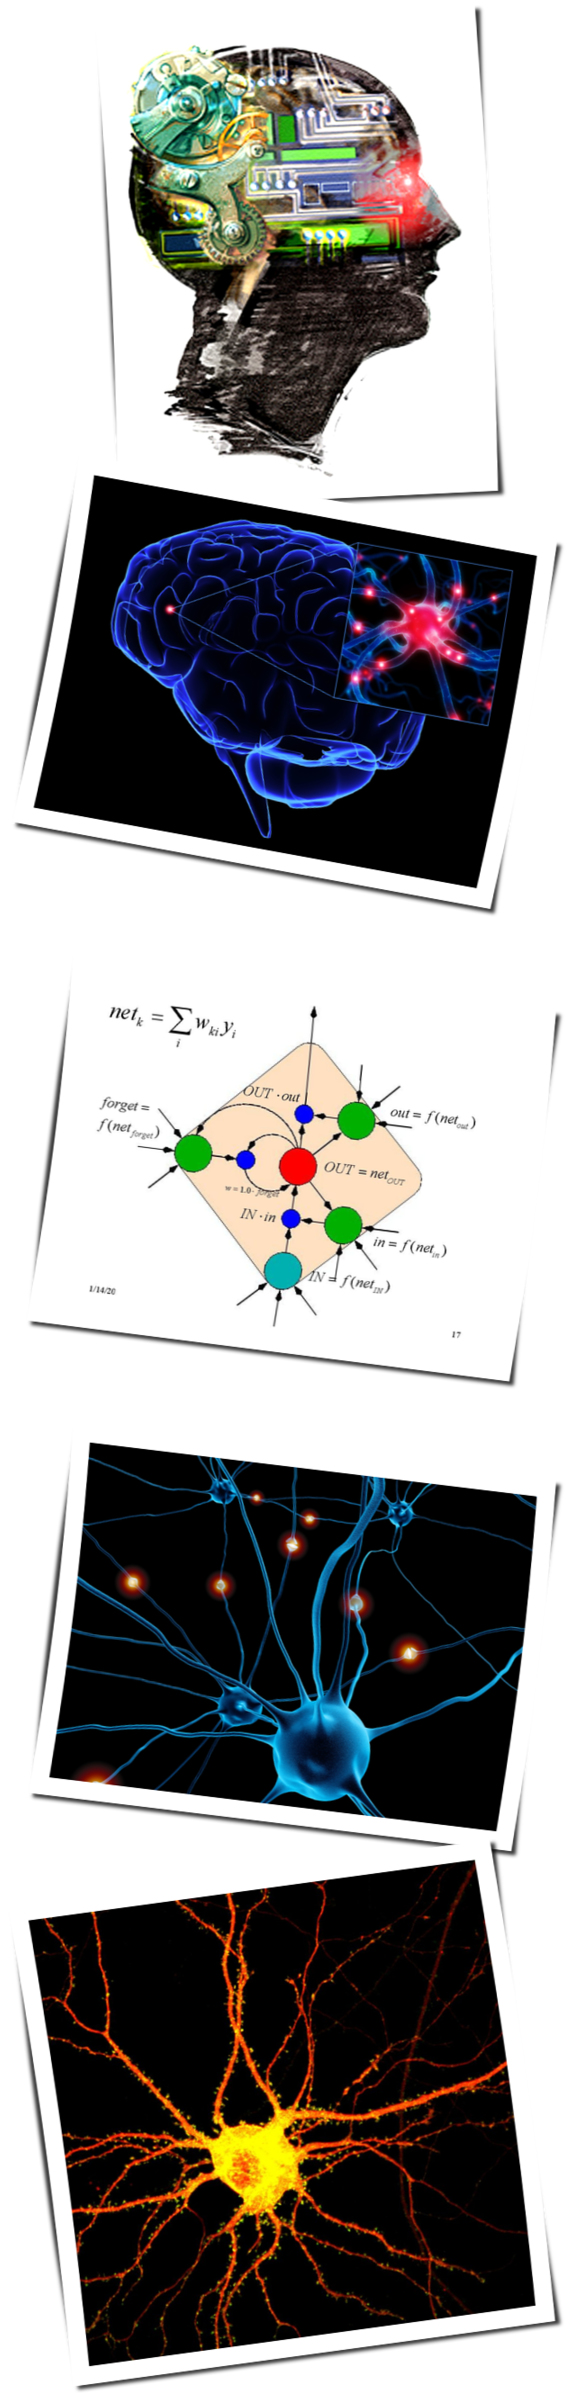
\includegraphics[width=0.17\paperwidth]{graphics/nn.jpg}};
}

\DeclareMathOperator*{\argmax}{arg\,max}


\newcommand{\vect}[1]{\boldsymbol{#1}} % Uncomment for BOLD vectors.

\title{A quick introduction to machine learning\\
Spyros Samothrakis\\
Senior Lecturer, IADS\\
University of Essex\\
MiSoC}
\author{June 22, 2022}
\date{}

\begin{document}
\frame{\titlepage}


\section{}\label{section}

\usebackgroundtemplate{

}

\section{Introduction}\label{introduction}

\begin{frame}{Welcome/course contents}

\begin{itemize}
\tightlist
\item
  What will this course cover?

  \begin{itemize}
  \tightlist
  \item
    Day 1: An intro to machine learning (ML)
  \item
    Day 1: ML labs
  \item
    Day 2: An intro to causal inference
  \item
    Day 2: ML and causal inference labs
  \end{itemize}
\item
  Textbooks?

  \begin{itemize}
  \item
    \href{http://www.cs.cmu.edu/~tom/mlbook.html}{Mitchell, T. M.
    (1997). Machine learning.}
  \item
    \href{https://www.microsoft.com/en-us/research/publication/pattern-recognition-machine-learning/}{Bishop,
    C. M. (2006). Pattern recognition and machine learning. springer.}
  \item
    \href{http://www.stat.cmu.edu/~larry/all-of-statistics/index.html}{Wasserman,
    L. (2013). All of statistics: a concise course in statistical
    inference. Springer Science \& Business Media.}
  \end{itemize}
\end{itemize}

\end{frame}

\begin{frame}{Better science through data}

\href{http://languagelog.ldc.upenn.edu/myl/JimGrayOnE-Science.pdf}{Hey,
Tony, Stewart Tansley, and Kristin M. Tolle. ``Jim Gray on eScience: a
transformed scientific method.'' (2009).}

\begin{itemize}
\tightlist
\item
  Thousand years ago: empirical branch

  \begin{itemize}
  \tightlist
  \item
    You observed stuff and you wrote down about it
  \end{itemize}
\item
  Last few hundred years: theoretical branch

  \begin{itemize}
  \tightlist
  \item
    Equations of gravity, equations of electromagnetism
  \end{itemize}
\item
  Last few decades: computational branch

  \begin{itemize}
  \tightlist
  \item
    Modelling at the micro level, observing at the macro level
  \end{itemize}
\item
  Today: data exploration

  \begin{itemize}
  \tightlist
  \item
    Let machines create models using vast amounts of data
  \end{itemize}
\end{itemize}

\end{frame}

\begin{frame}{Better business through data}

\begin{itemize}
\tightlist
\item
  There was a report by Mckinsey
\end{itemize}

\href{http://www.mckinsey.com/business-functions/digital-mckinsey/our-insights/big-data-the-next-frontier-for-innovation}{Manyika,
J., Chui, M., Brown, B., Bughin, J., Dobbs, R., Roxburgh, C., \& Hung
Byers, A. (2011). Big data: The next frontier for innovation,
competition, and productivity. McKinsey Global Institute.}

\begin{itemize}
\tightlist
\item
  Urges everyone to monetise ``Big Data''
\item
  Use the data provided within your organisation to gain insights
\item
  Has some numbers as to how much this is worth
\item
  Proposes a number of methods, most of them associated with machine
  learning and databases
\end{itemize}

\end{frame}

\begin{frame}{Why is it popular now?}

\begin{itemize}
\item
  \textbf{Algorithms + data + tools}
\item
  \href{http://projecteuclid.org/download/pdf_1/euclid.ss/1009213726\%20}{Breiman,
  L. (2001). Statistical modeling: The two cultures (with comments and a
  rejoinder by the author). Statistical science, 16(3), 199-231.}
\item
  \href{https://www.tkm.kit.edu/downloads/TKM1_2011_more_is_different_PWA.pdf}{Anderson,
  P. W. (1972). More is different. Science, 177(4047), 393-396.}
\item
  \href{https://www.jmlr.org/papers/volume12/pedregosa11a/pedregosa11a.pdf}{Pedregosa,
  et.al. (2011). Scikit-learn: Machine learning in Python. the Journal
  of machine Learning research, 12, 2825-2830.}
\end{itemize}

\end{frame}

\begin{frame}{So this course covers tools}

\begin{itemize}
\tightlist
\item
  ML theory

  \begin{itemize}
  \tightlist
  \item
    \emph{Supervised learning} \emph{Regression} \emph{Classification}
  \item
    Understanding basic modelling
  \item
    Confirming your model is sane
  \item
    Tuning your model
  \item
    \textbf{All within a very applied setting}
  \end{itemize}
\item
  Tools

  \begin{itemize}
  \tightlist
  \item
    Numpy
  \item
    Scikit-learn
  \end{itemize}
\end{itemize}

\end{frame}

\begin{frame}{What is supervised learning?}

\begin{itemize}
\tightlist
\item
  Imagine someone gives you a group of smokers

  \begin{itemize}
  \tightlist
  \item
    And asks the question -- what is their life expectancy?
  \end{itemize}
\item
  \textbf{Completely made up imaginary data}
\end{itemize}

\end{frame}

\begin{frame}{Some abstraction}

\begin{itemize}
\tightlist
\item
  We are given inputs \(x_0, x_1...x_n\) and we are looking to predict
  \(y\)
\item
  Let's plot!
\end{itemize}

\end{frame}

\begin{frame}{Regression - link the dots (1)}

\includegraphics[trim={0 0 0 0},clip,width = 0.9\textwidth]{./code/cropped/{intra_spiral_50-crop}.jpg}

\end{frame}

\begin{frame}{Regression - link the dots (2)}

\includegraphics[trim={0 0 0 0},clip,width = 0.9\textwidth]{./code/cropped/{intra_spiral_100-crop}.jpg}

\end{frame}

\begin{frame}{Regression - link the dots (3)}

\includegraphics[trim={0 0 0 0},clip,width = 0.9\textwidth]{./code/cropped/{intra_spiral_200-crop}.jpg}

\end{frame}

\begin{frame}{Regression - link the dots (4)}

\includegraphics[trim={0 0 0 0},clip,width = 0.9\textwidth]{./code/cropped/{intra_spiral_500-crop}.jpg}

\end{frame}

\begin{frame}{Regression - link the dots (5)}

\includegraphics[trim={0 0 0 0},clip,width = 0.9\textwidth]{./code/cropped/{intra_spiral_1000-crop}.jpg}

\end{frame}

\begin{frame}{Regression - link the dots (6)}

\includegraphics[trim={0 0 0 0},clip,width = 0.9\textwidth]{./code/cropped/{intra_spiral_10000-crop}.jpg}

\end{frame}

\begin{frame}{Classification - draw a boundary (1)}

\includegraphics[trim={0 0 0 0},clip,width = 0.9\textwidth]{./code/cropped/{intra_spiral_50_class-crop}.jpg}

\end{frame}

\begin{frame}{Classification - draw a boundary (2)}

\includegraphics[trim={0 0 0 0},clip,width = 0.9\textwidth]{./code/cropped/{intra_spiral_100_class-crop}.jpg}

\end{frame}

\begin{frame}{Classification - draw a boundary (3)}

\includegraphics[trim={0 0 0 0},clip,width = 0.9\textwidth]{./code/cropped/{intra_spiral_200_class-crop}.jpg}

\end{frame}

\begin{frame}{Classification - draw a boundary (4)}

\includegraphics[trim={0 0 0 0},clip,width = 0.9\textwidth]{./code/cropped/{intra_spiral_500_class-crop}.jpg}

\end{frame}

\begin{frame}{Classification - draw a boundary (5)}

\includegraphics[trim={0 0 0 0},clip,width = 0.9\textwidth]{./code/cropped/{intra_spiral_1000_class-crop}.jpg}

\end{frame}

\begin{frame}{Classification - draw a boundary (6)}

\includegraphics[trim={0 0 0 0},clip,width = 0.9\textwidth]{./code/cropped/{intra_spiral_10000_class-crop}.jpg}

\end{frame}

\begin{frame}{Full data}

\includegraphics[trim={0 0 0 0},clip,width = 0.9\textwidth]{./code/cropped/{extra_spiral-crop}.pdf}

\end{frame}

\begin{frame}{Intuition}

\begin{itemize}
\tightlist
\item
  That's it - we are given data, and we need to come up with an
  algorithm to join it up -- but in high dimensions

  \begin{itemize}
  \tightlist
  \item
    Can can be binary, categorical, real-valued
  \end{itemize}
\item
  How well well a function joins the data is called the ``loss''
\item
  Very low loss is not good, it might not generalise that well to unseen
  data points -- you can learn to memorise data instances
\end{itemize}

\end{frame}

\section{Classic algorithms for joining those
dots}\label{classic-algorithms-for-joining-those-dots}

\begin{frame}{Linear regression}

\begin{itemize}
\tightlist
\item
  Linear and logistic regression

  \begin{itemize}
  \tightlist
  \item
    Logistic regression does classification
  \end{itemize}
\item
  You just assume everything is a line
\end{itemize}

\end{frame}

\begin{frame}{Example (Linear regression)}

\includegraphics[trim={0 0 0 0},clip,width = 0.9\textwidth]{./code/cropped/{reg_intra_spiral_200_LinearRegression-crop}.jpg}

\end{frame}

\begin{frame}{Example (Linear regression)}

\includegraphics[trim={0 0 0 0},clip,width = 0.9\textwidth]{./code/cropped/{reg_intra_spiral_2000_LinearRegression-crop}.jpg}

\end{frame}

\begin{frame}{Example (Decision tree)}

\includegraphics[trim={0 0 0 0},clip,width = 0.9\textwidth]{./code/cropped/{reg_intra_spiral_200_DecisionTreeRegressor-crop}.jpg}

\end{frame}

\begin{frame}{Example (Decision tree)}

\includegraphics[trim={0 0 0 0},clip,width = 0.9\textwidth]{./code/cropped/{reg_intra_spiral_2000_DecisionTreeRegressor-crop}.jpg}

\end{frame}

\begin{frame}{Example (Decision tree --- internal)}

\includegraphics[trim={0 0 0 0},clip,width = 0.3\textwidth]{./code/cropped/{reg_vis_tree_intra_spiral_2000_DecisionTreeRegressor-crop}.jpg}

\end{frame}

\begin{frame}{Example (Random forest)}

\includegraphics[trim={0 0 0 0},clip,width = 0.9\textwidth]{./code/cropped/{reg_intra_spiral_2000_RandomForestRegressor-crop}.jpg}

\end{frame}

\begin{frame}{Example (Random forest)}

\includegraphics[trim={0 0 0 0},clip,width = 0.9\textwidth]{./code/cropped/{reg_intra_spiral_2000_RandomForestRegressor-crop}.jpg}

\end{frame}

\begin{frame}{Example (Random forest)}

\includegraphics[trim={0 0 0 0},clip,width = 0.9\textwidth]{./code/cropped/{reg_intra_spiral_2000_CatBoostRegressor-crop}.jpg}

\end{frame}

\begin{frame}{Example (Gradient boosting)}

\includegraphics[trim={0 0 0 0},clip,width = 0.9\textwidth]{./code/cropped/{reg_intra_spiral_2000_CatBoostRegressor-crop}.jpg}

\end{frame}

\begin{frame}{Classification (Decision trees)}

\includegraphics[trim={0 0 0 0},clip,width = 0.9\textwidth]{./code/cropped/{class_spiral_DecisionTreeClassifier}.png}

\end{frame}

\begin{frame}{Classification (Random forests)}

\includegraphics[trim={0 0 0 0},clip,width = 0.9\textwidth]{./code/cropped/{class_spiral_RandomForestClassifier}.png}

\end{frame}

\section{Higher dimensions}\label{higher-dimensions}

\begin{frame}{Until now}

\end{frame}

\section{Testin'}\label{testin}

\begin{frame}{But how do we know this will generalise well?}

\begin{itemize}
\tightlist
\item
  Train/Validation/Test split
\item
  Cross validation
\end{itemize}

\end{frame}

\section{Tuning}\label{tuning}

\begin{frame}{Hyperparameters}

\begin{itemize}
\tightlist
\item
  How many trees?
\item
  Tree depth?
\item
  l2?
\end{itemize}

\end{frame}

\section{Wrapping up}\label{wrapping-up}

\end{document}
